\documentclass[9pt]{article}

\usepackage{amssymb}
\usepackage{amsmath}
\usepackage{amsfonts}
\usepackage{comment}
\usepackage{fancyhdr}
\usepackage{mathrsfs}
\usepackage{enumitem}
\usepackage{graphicx}

\usepackage{tikz}

\voffset = -50pt
%\textheight = 700pt
\addtolength{\textwidth}{60pt}
\addtolength{\evensidemargin}{-30pt}
\addtolength{\oddsidemargin}{-30pt}
%\setlength{\headheight}{44pt}

\newcommand{\qed}{\hfill \ensuremath{\Box}}


\newcommand*\circled[1]{\tikz[baseline=(char.base)]{
            \node[shape=circle,draw,inner sep=2pt] (char) {#1};}}

\newcommand{\Z}{\mathbb{Z}}
\newcommand{\I}{\mathbb{I}}
\newcommand{\M}{\mathbb{M}}
\newcommand{\R}{\mathbb{R}}
\newcommand{\C}{\mathbb{C}}
%\setcounter{section}{-1}

\begin{document}
\topskip0pt
\vspace*{\fill}
\begin{center}
{\Huge \begin{tabular}{@{}ll@{}}
   Class: & CECS 201, Section 7 \\ \\ \\
   Lab: & 7 \\ \\ \\
   Title: & 7 Segment Decoder \\ \\ \\
   Student Name: & Barry Joseph Okonoboh \\ \\ \\
   Due Date: & 11:59:59 P.M., 23, March 2015 \\ \\ \\
   Instructor: & Dan Cregg
\end{tabular}}
\end{center}
\vspace*{\fill}
\newpage
\begin{enumerate}
%%%%%%%%%%%%%%%%%%%%%%%%%%%%%%%%%%%%%%%%01%%%%%%%%%%%%%%%%%%%%%%%%%%%%%%%%%%%%%%
   \item[b.] \textbf{Introduction.} In this lab we create a 4-binary input to a
              7 segment LED Binary to Hexidecimal decoder.
   \item[c.] \textbf{Project Description.} An led contains 7 segment, each of
             which can be in the on (0) or off (1) state. The state of each 
             segment depends on the character that is currently being displayed. 
             In this lab, we are interested in the 16 hexadecimal characters 
             namely:
             $$0, 1, 2, 3, 4, 5, 6, 7, 8, 9 A, b, C, d, E, F.$$
             Each of these characters maps to a unique input, and the truth 
             table below shows the segments that are on and off for these 
             characters.

             The ledEnable output ensures that only a character whose binary 
             input contains at least a 1 is displayed; that is, only 0 is not
             displayed.

  	\item[d.] \textbf{Schematic.}
             \begin{center}
                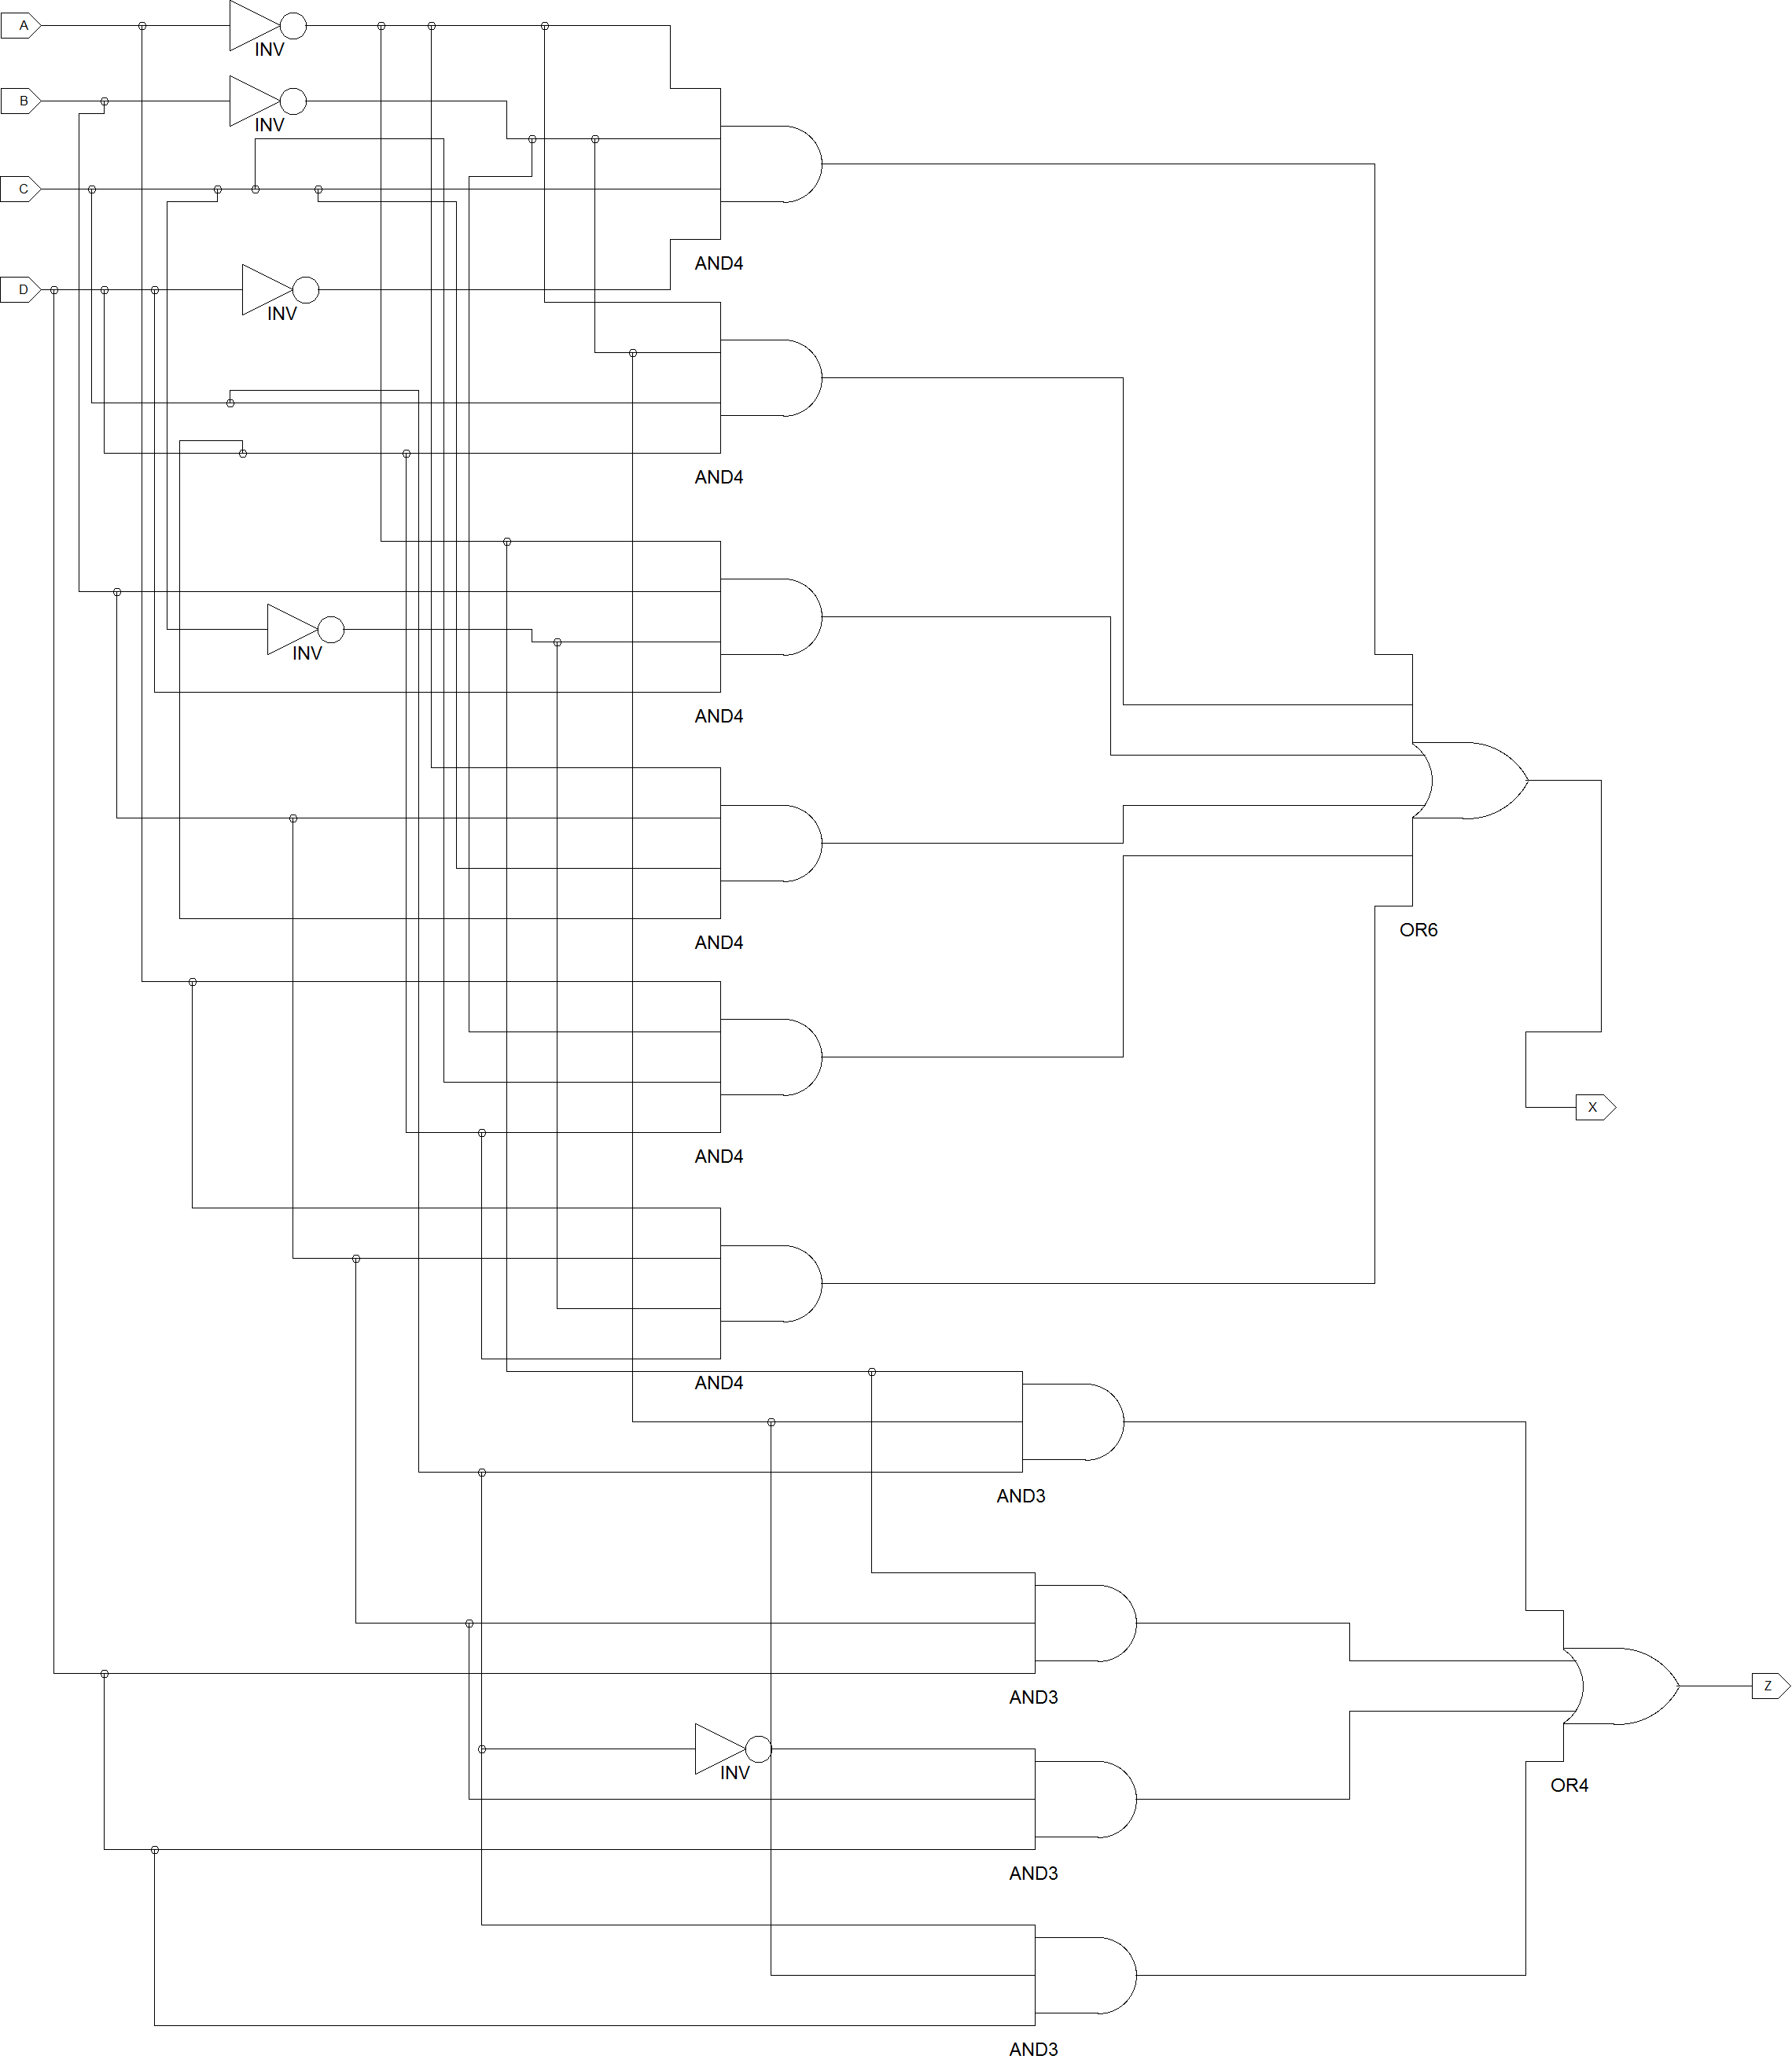
\includegraphics[width=\textwidth]{schematic.png}
             \end{center}
             
             \textbf{Truth Table.}   
   
   \begin{center}
    \begin{tabular}{@{}|c|c|c|c|c|c|c|c|c|c|c|c|@{}}
   \hline
         $A$ & $B$ & $C$ & $D$ & ledA & ledB & ledC & ledD & ledE & ledF & ledG
             & ledEnable \\ \hline
         0 & 0 & 0 & 0 & 0 & 0 & 0 & 0 & 0 & 0 & 1 & 1 \\ \hline
         0 & 0 & 0 & 1 & 1 & 0 & 0 & 1 & 1 & 1 & 1 & 0 \\ \hline
         0 & 0 & 1 & 0 & 0 & 0 & 1 & 0 & 0 & 1 & 0 & 0 \\ \hline
         0 & 0 & 1 & 1 & 0 & 0 & 0 & 0 & 1 & 1 & 0 & 0 \\ \hline
         0 & 1 & 0 & 0 & 1 & 0 & 0 & 1 & 1 & 0 & 0 & 0 \\ \hline
         0 & 1 & 0 & 1 & 0 & 1 & 0 & 0 & 1 & 0 & 0 & 0 \\ \hline
         0 & 1 & 1 & 0 & 0 & 1 & 0 & 0 & 0 & 0 & 0 & 0 \\ \hline
         0 & 1 & 1 & 1 & 0 & 0 & 0 & 1 & 1 & 1 & 1 & 0 \\ \hline
         1 & 0 & 0 & 0 & 0 & 0 & 0 & 0 & 0 & 0 & 0 & 0 \\ \hline
         1 & 0 & 0 & 1 & 0 & 0 & 0 & 0 & 1 & 0 & 0 & 0 \\ \hline
         1 & 0 & 1 & 0 & 0 & 0 & 0 & 1 & 0 & 0 & 0 & 0 \\ \hline
         1 & 0 & 1 & 1 & 1 & 1 & 0 & 0 & 0 & 0 & 0 & 0 \\ \hline
         1 & 1 & 0 & 0 & 0 & 1 & 1 & 0 & 0 & 0 & 1 & 0 \\ \hline
         1 & 1 & 0 & 1 & 1 & 0 & 0 & 0 & 0 & 1 & 0 & 0 \\ \hline
         1 & 1 & 1 & 0 & 0 & 1 & 1 & 0 & 0 & 0 & 0 & 0 \\ \hline
         1 & 1 & 1 & 1 & 0 & 1 & 1 & 1 & 0 & 0 & 0 & 0 \\ \hline
\end{tabular}
   \end{center}
\end{enumerate}
\end{document}
